\newpage
\section{Stosowane technologie i narzędzia}
W erze postępującej technologii, chatboty przekształciły się z prostych narzędzi automatycznych odpowiedzi w zaawansowane systemy oparte na sztucznej inteligencji, oferując bardziej naturalne i płynne interakcje. Na rynku pojawia się coraz więcej zaawansowanych rozwiązań opartych na dużych modelach językowych (LLM), które radykalnie zmieniają sposób, w jaki ludzie komunikują się z maszynami.

Na tym tle wyłoniła się klasa Agentów AI - autonomicznych systemów, które, wykorzystując możliwości LLM, potrafią planować działania, podejmować decyzje, korzystać z narzędzi i współpracować w ramach złożonych przepływów
pracy. Zdolność do pracy w kontekście, iteracyjnego usprawniania wyników i adaptacji do zmieniających się warunków otwiera nowe możliwości w automatyzacji procesów oraz wspomaganiu decyzji, w tym wytwarzaniu oprogramowania.

W niniejszym rozdziale przedstawiono stosowane technologie i narzędzia wspierające implementację systemów agentowych: interfejsy API, biblioteki i środowiska ułatwiające integrację modeli oraz koordynację ich działań w konfiguracjach jednoagentowych i wieloagentowych.

\subsection{Wykorzystane biblioteki}
W ramach pracy wykorzystano dwa nowoczesne narzędzia wspierające projektowanie i uruchamianie systemów agentowych w
środowisku programistycznym:
\begin{itemize}
  \item \textbf{OpenAI Agents} \textendash\  biblioteka i API umożliwiające definiowanie agentów, ich ról oraz dostępnych narzędzi (Function Calling), a także zarządzanie pamięcią i kontekstem rozmowy. Została użyta do orkiestracji zadań, integracji narzędzi programistycznych oraz koordynacji przepływu informacji między agentami w konfiguracjach jedno- i wieloagentowych.
  \item \textbf{Claude Code} \textendash\  narzędzie ukierunkowane na pracę z kodem, wspierające analizę repozytorium, modyfikacje plików i iteracyjne wykonywanie zadań programistycznych z zachowaniem kontroli użytkownika. Wykorzystano je do wsparcia procesu implementacji  refaktoryzacji, w szczególności przy zadaniach wymagających kontekstu całego projektu oraz precyzyjnych zmian w wielu plikach.
\end{itemize}

Wybór powyższych narzędzi był motywowany ich dojrzałością ekosystemową oraz wsparciem dla wzorców pracy agentowej zorientowanej na zadania, co umożliwiło szybkie prototypowanie przepływów i powtarzalne eksperymenty.

\subsection{Zastosowane konfiguracje systemu agentowego}
W ramach niniejszej pracy przeprowadzono serię eksperymentów mających na celu empiryczną ocenę wpływu różnych konfiguracji
systemów agentowych na proces tworzenia oprogramowania. Badania koncentrowały się na porównaniu trzech kluczowych architektur:
\begin{itemize}
    \item \textbf{Konfiguracja A - Pojedynczy Agent} (Programista) - system z jednym agentem pełniącym wszystkie role
    \item \textbf{Konfiguracja B - System Dwuagentowy} (Programista-Architekt) - współpraca dwóch wyspecjalizowanych agentów
    \item \textbf{Konfiguracja C - System Trójagentowy} (Programista-Architekt-Tester) - zespół trzech agentów z podziałem odpowiedzialności
\end{itemize}

Każda z konfiguracji została przetestowana w czterech kluczowych kategoriach związanych z wytwarzaniem oprogramowania, wykorzystując model GPT-5 oraz Claude Opus 4 jako fundamentalne modele językowe. Eksperymenty przeprowadzono w kontrolowanym środowisku, gdzie każda konfiguracja otrzymywała identyczne zadania do wykonania. Szczególną uwagę zwrócono na różnice w jakości generowanego kodu, czasie wykonania zadań oraz efektywności współpracy między agentami.

Wybór tych konkretnych konfiguracji był podyktowany chęcią zbadania, jak stopniowe zwiększanie złożoności systemu agentowego oraz zadanej aplikacji wpływa na efektywność procesu wytwarzania oprogramowania. Konfiguracja A reprezentuje najprostsze podejście, gdzie jeden agent musi poradzić sobie ze wszystkimi aspektami zadania. Konfiguracja B wprowadza podział na role koncepcyjne (architekt) i implementacyjne (programista). Konfiguracja C dodatkowo wyodrębnia rolę kontroli jakości (tester), tworząc pełniejszy cykl wytwarzania oprogramowania.

\subsubsection*{Architektura pojedynczego agenta}
Najprostsza konfiguracja wykorzystywała pojedynczego agenta opartego na modelu językowym,  który pełnił wszystkie role — od analizy wymagań po generowanie kodu.  Agent ten korzystał z zestawu narzędzi, używając Function Calling, aby odczytywać pliki specyfikacji, projektować rozwiązania oraz pisać pliki kodu aplikacji.

\begin{figure}[!h]
    \centering 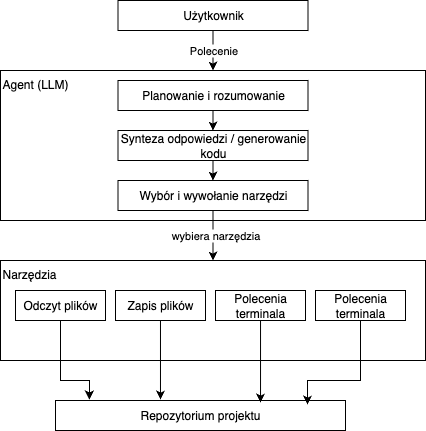
\includegraphics[width=0.8\linewidth]{img/architektura-agent.png}
    \caption{Architektura pojedynczego agenta}
    \label{fig:architektura-pojedynczego-agenta}
\end{figure}

Na rysunku \ref{fig:architektura-pojedynczego-agenta} pokazano minimalny przepływ pracy w eksperymentach dla jednego agenta. Agent otrzymuje wejście (prompt/specyfikację), następnie tworzy plan działania (kroki i artefakty), po czym iteracyjnie korzysta z narzędzi do odczytu istniejących plików i zapisu nowych zmian w repozytorium. Agent sprawdza zgodność wygenerowanego kodu z planem i wymaganiami, aktualizuje plan w razie niespójności i generuje kod.

\subsubsection*{Architektura dwuagentowa (architekt-programista)}
W tej konfiguracji wykorzystano:
\begin{itemize}
    \item \textbf{Agent Architekt} - odpowiedzialny za analizę wymagań, projektowanie struktury aplikacji i podział zadań. Używa narzędzi do odczytania specyfikacji aplikacji
    \item \textbf{Agent Programista} - implementujący kod według wytycznych architekta. Używa zestaw narzędzi do odczytywania i pisania plików jak i do wykonywania poleceń w terminalu.
\end{itemize}

\begin{figure}[!h]
    \centering 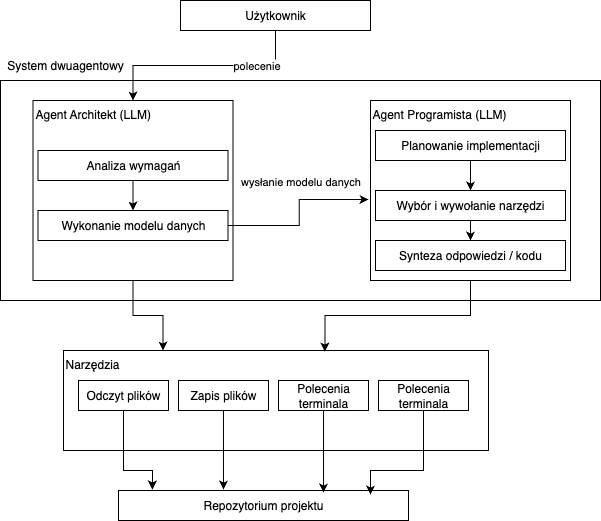
\includegraphics[width=0.9\linewidth]{img/architektura-agent-architekt.png}
    \caption{Architektura dwuagentowa: Architekt-Programista}
    \label{fig:architektura-dwuagentowa}
\end{figure}

Na rysunku \ref{fig:architektura-dwuagentowa} zilustrowano współpracę Architekta i Programisty.
Architekt rozpoczyna od analizy wejścia i tworzy artefakty koncepcyjne: proponowany model danych aplikacji. Następnie przekazuje je Programiście, który implementuje zmiany, używając Function Calling do edycji plików i wykonywania komend pomocniczych (np. formatowanie, generowanie szablonów). Komunikacja odbywa się poprzez dostęp do aktualnego repozytorium projektu, co umożliwia śledzenie kontekstu i decyzji. Proces kończy się, gdy Programista wygeneruje kod aplikacji.

\subsubsection*{Architektura wieloagentowa}
Najbardziej złożona konfiguracja obejmowała zespół wyspecjalizowanych agentów:
\begin{itemize}
    \item \textbf{Produkt Manager} - interpretacja wymagań biznesowych, utworzenie zadań i podzielenie między zespołem
    \item \textbf{Architekt systemu} - projektowanie architektury i modelu danych
    \item \textbf{Programista} - implementacja aplikacji
    \item \textbf{Recenzent kodu} - przegląd kodu i sugestie ulepszeń
\end{itemize}

\begin{figure}[!h]
    \centering 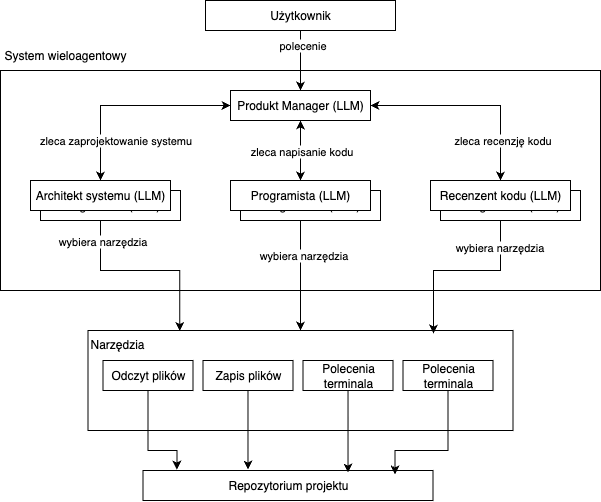
\includegraphics[width=0.9\linewidth]{img/architektura-wieloagentowa.png}
    \caption{Architektura wieloagentowa}
    \label{fig:architektura-wieloagentowa}
\end{figure}

Na rysunku \ref{fig:architektura-wieloagentowa} przedstawiono pełniejszy cykl z podziałem ról. Product Manager przyjmuje polecenie użytkownika, porządkuje wymagania i tworzy backlog zadań, Architekt definiuje model danych, Programista implementuje, a Recenzent dokonuje przeglądu zmian i zgłasza uwagi. Iteracje mają charakter bramek jakościowych: implementacja trafia do przeglądu, po akceptacji przechodzi dalej; w razie zastrzeżeń wraca do Programisty z konkretnymi poprawkami. W eksperymentach zapewniono te same wejścia, limity kroków i dostęp do narzędzi dla wszystkich konfiguracji, aby różnice w wynikach wynikały z organizacji pracy agentów, a nie z warunków testu. Zakończenie następuje po realizacji zadań oraz pozytywnej weryfikacji Recenzenta.

Koordynacja między agentami była realizowana poprzez bibliotekę OpenAI Agents SDK \cite{openai_agents_sdk_python_2025} z wykorzystaniem wzorca asynchronicznego \cite{mmazurekPythonProgramowanieAsynchroniczne} między agentami.

\clearpage